\section{Analysis}

The main focus of our project was finding out whether the election of Donald Trump had an impact on suicide rates in the United States of America.
To that end, the first diagramm we created was simply a bar chart with the total amount of suicides in the United States of America per year for the years we had data on: 1999 through 2017.

\begin{figure}[tb]
\centering
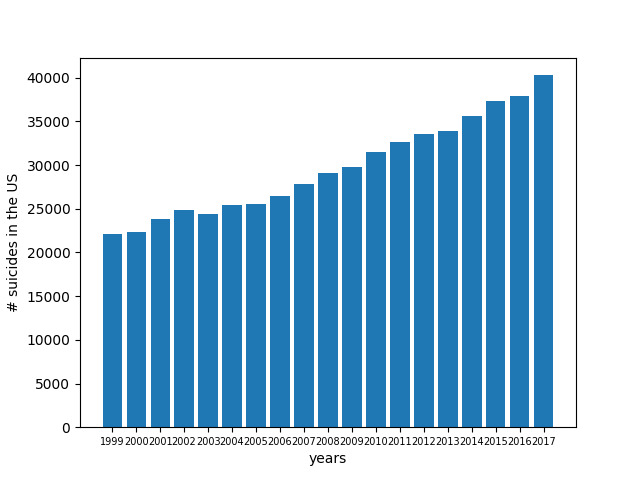
\includegraphics[width=0.85\textwidth]{g9-suicides_per_year}
\caption{Total yearly suicides in the US from 1999 to 2017.}
\label{fig:yearly_suicides}
\end{figure}

This diagramm can be found in \Cref{fig:yearly_suicides}. As can be plainly seen, there was a marked uptick in suicides between 2016 and 2017.
Since Donald Trump was elected president near the end of 2016 on the 8th of November and assumed the presidency in the beginning of 2017 on the 20th of January, this noticeable jump provides us with some tentative evidence in support of our hypothesis.
\par

\begin{figure}[tb]
\centering
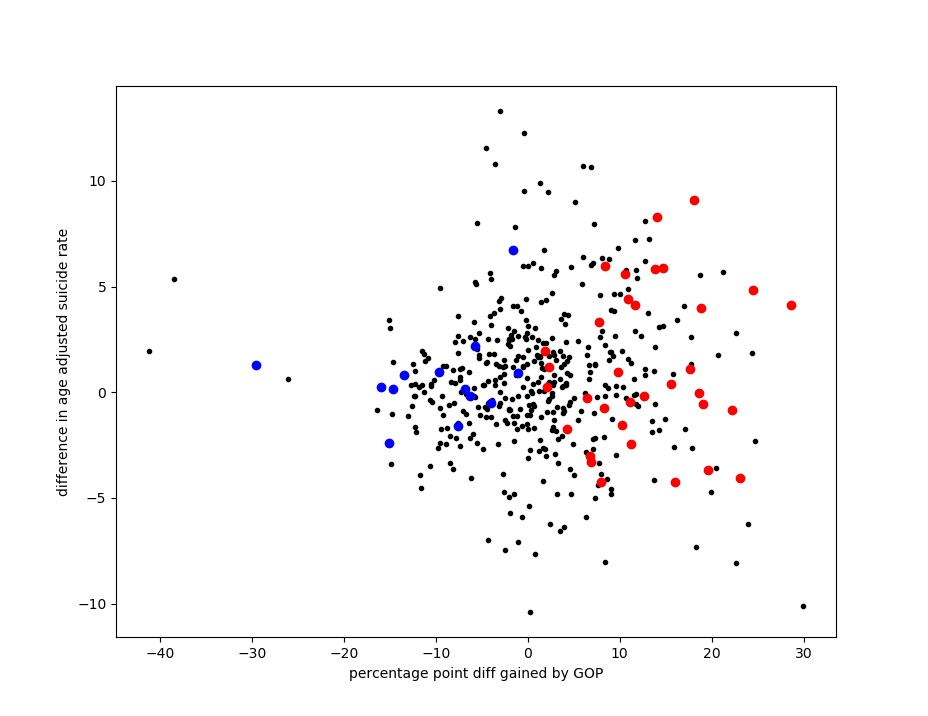
\includegraphics[width=0.85\textwidth]{g9-suicides-diff-votes-diff}
\caption{Difference in age adjusted suicide rate per US county between 2016 and 2017 plotted against the gain by the republican party over the democratic party from 2012 to 2016. Counties that flipped from democratic to republican are highlighted in red, those where the reverse happened are marked blue.}
\label{fig:suicides-diff-votes-diff}
\end{figure}

However, the diagramm in \Cref{fig:suicides-diff-votes-diff} shows that there was no notable correlation on a county level between how much better Trump performed than Mitt Romney did in 2012 and the increase in suicides in said county.
Even looking at the counties which flipped during the 2016 election yields no discernable correlation.
What can be made out is that, in most counties, Trump did better than Romney did in 2012 and suicide rates rose.
These findings are not in the least bit surprising, given that Trump won the election and Romney did not and that the total amount of suicides rose markedly, but it's good to see that our data reflects reality and is consistent.

\begin{figure}[tb]
\centering
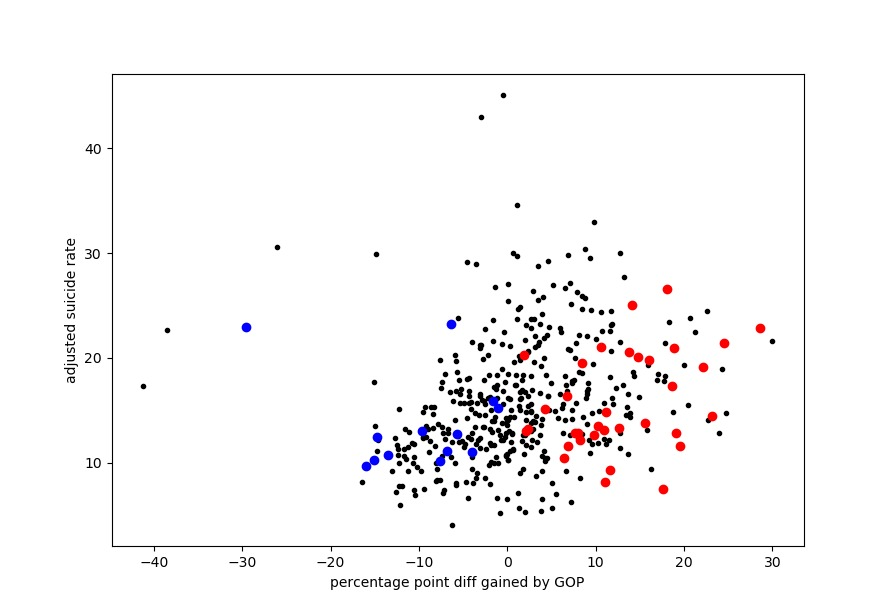
\includegraphics[width=0.85\textwidth]{g9-suicides-votes-diff}
\caption{Age adjusted suicide rate per US county in 2016 plotted against the gain by the republican party over the democratic party from 2012 to 2016. Counties that flipped from democratic to republican are highlighted in red, those where the reverse happened are marked blue.}
\label{fig:suicides-votes-diff}
\end{figure}

\par
\Cref{fig:suicides-votes-diff} shows a similar picture, but uses the age adjusted suicide rate in 2016 instead of the increase between 2016 and 2017.
In this diagramm we see a noticeable, if slight, correlation.
It seems like Trump did unexpectedly well compared to establishment republican candidate Romney in counties with high suicide rates.
\cite{goldman2018} came to a similar finding when they examined the relation between life expectancy and republican gains in the 2016 election.
This is an interesting finding in its own right, but does not support our hypothesis.
It is however worth noting, that it in no way explains the rise in suicides between 2016 and 2017.

\begin{figure}[tb]
\centering
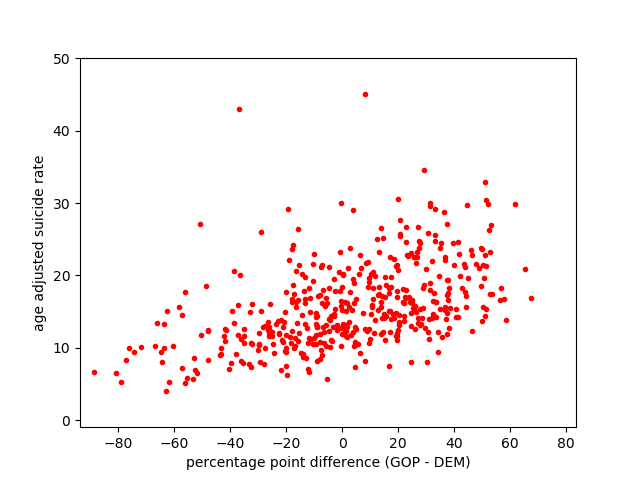
\includegraphics[width=0.85\textwidth]{g9-suicides-votes}
\caption{Age adjusted suicide rate per US county in 2017 plotted against the percentage point difference between the GOP and the DNC in the 2016 presidential election.}
\label{fig:suicides-votes}
\end{figure}

\par
\Cref{fig:suicides-votes} contains a single frame of an animated scatter plot showing both the change in age adjusted suicide rate and the election results dynamically.
The animation did not reveal any unexpected or noteworthy insights into the data.
This still image, showing the election results in 2016 plotted against the suicide rate in 2017 does show, however, that there is a clear correlation between counties with a large portion of republican voters and high suicide rates.
The picture looks virtually the same when comparing the suicide rates in 2016 and the election results from 2012.
This tells us that Trumps success in counties with high suicide rates does not necessarily set him apart as a candidate.
It also suggests that the increased suicide rate since 2012 might explain some of his success, and not the other way around.

\begin{figure}[tb]
\centering
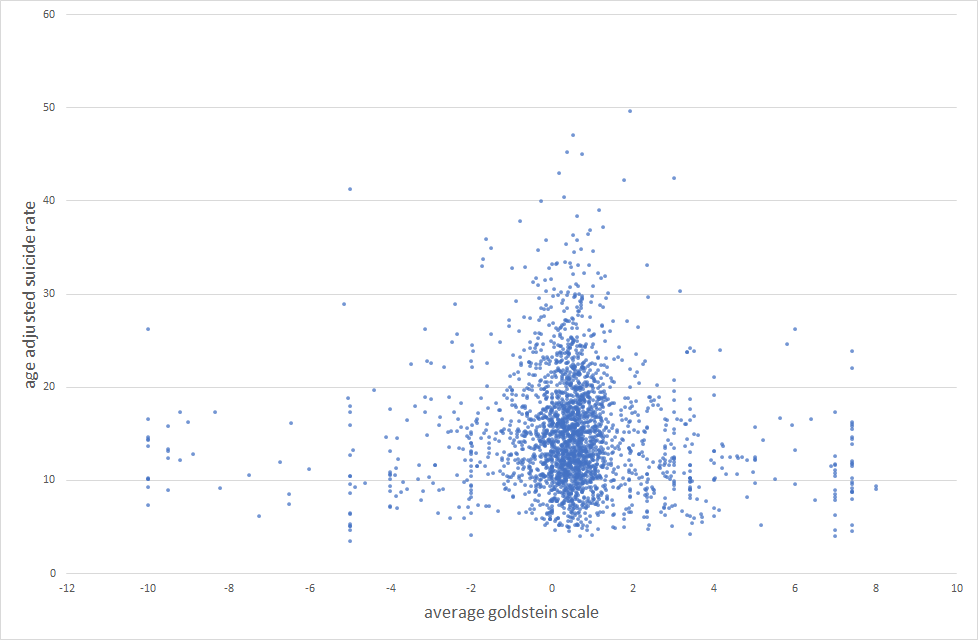
\includegraphics[width=0.85\textwidth]{g9-suicides-gdelt}
\caption{Age adjusted yearly suicide rate per US county plotted against the average goldstein scale of all events which took place according to GDELT.}
\label{fig:suicides-gdelt}
\end{figure}

\par
Finally, \Cref{fig:suicides-gdelt} shows the suicide rates for each county for each year (if data was available) in relation to the average goldstein scale of all events which took place in the county during that year.
A positive goldstein scale is supposed to signify that the event is expected to have a positive effect, a negative value therefor represents bad news.
As can be plainly seen, there is very little correlation.

\subsection{Methods}

We generated all diagramms by performing SQL queries on our database and used python with matplotlib do visualize the data.
The data for \Cref{fig:yearly_suicides} was selected using the following straightforward query:

\begin{lstlisting}[language=SQL]
SELECT
    year, SUM(deaths)
FROM 
    suiciderate
GROUP BY
    year 
ORDER BY
    year
;
\end{lstlisting}

\Cref{fig:suicides-diff-votes-diff}, \Cref{fig:suicides-votes-diff}, \Cref{fig:suicides-votes} were all created using the results of the same query:

\begin{lstlisting}[language=SQL]
SELECT
    county.name, county.state_name,
    100 * cast(e2012.votesgop - e2012.votesdem as decimal)
        /(e2012.votesgop + e2012.votesdem + e2012.votesother) 
        AS perdiff2012,
    100 * cast(e2016.votesgop - e2016.votesdem as decimal)
        /(e2016.votesgop + e2016.votesdem + e2016.votesother) 
        AS perdiff2016,
    s2016.ageadjustedrate AS rate2016,
    s2017.ageadjustedrate AS rate2017
FROM
    county
    JOIN electionresult e2012 ON 
        e2012.countygeoid = county.gid AND e2012.year = 2012
    JOIN electionresult e2016 ON 
        e2016.countygeoid = county.gid AND e2016.year = 2016
    JOIN suiciderate s2016 ON 
        s2016.countygeoid = county.gid AND s2016.year = 2016
    JOIN suiciderate s2017 ON 
        s2017.countygeoid = county.gid AND s2017.year = 2017
WHERE
    s2016.ageadjustedrate IS NOT NULL 
    AND s2017.ageadjustedrate IS NOT NULL
;
\end{lstlisting}

This query selects every US county for which we have associated suicide rate data and lection data for both 2012 and 2016.
Some counties had too few suicides or were perhaps not surveyed, so our source did not report an age adjusted suicide rate for them.
Using the results of this query, we could plot any combination of the election results in 2012, those in 2016 or the difference between the two and the age adjusted suicide rate in 2016, 2017 or the difference between the two.
In order to make the animation, we interpolated between the scatter plot of the 2012 election results and 2016 suicide rates and that of 2016 and 2016 repectively.
\par
In order to abtain the data for \Cref{fig:suicides-gdelt} we ran a similar query to find out to what degree the data in GDELT was able to explain the suicide rates:

\begin{lstlisting}[language=SQL]
SELECT
    county.name, county.state_name, ageadjustedrate, (
        SELECT
            AVG(goldsteinScale)
        FROM
            city
            JOIN "Event" e ON 
                e.actor2geoid = city.geoid 
                OR e.geoid = city.geoid
            JOIN "Action" a ON 
                a.id = e.actionid
        WHERE
            city.countygid = county.gid 
            AND EXTRACT(year FROM e.dateoccurred) 
                = sr.year
    )
FROM
    county
    JOIN suiciderate sr ON 
        sr.countygeoid = county.gid
WHERE
    sr.ageadjustedrate IS NOT NULL
;
\end{lstlisting}

Unfortunately, this query proved entirely too time consuming and was not finished running by the time the deadline of this report was approaching.
After the query had been running for several minutes, we took to using postgreSQL's EXPLAIN and ANALYZE functionality to look at the execution plan of the query and estimate how long it might take to finish.
The figure we came up with comparing the estimated cost by postgreSQL and comparing the cost of smaller queries to their actual runtime was about 250 hours.
We assumed culprit was a missing index on the dateoccurred field of the Event relation.
Because of this missing index, the execution plan involved performing a sequential scan of our biggest table with hundreds of millions of entries inside a nested loop.
We added this missing index but the execution plan remained the same.
As a second measure, we added a year field to the Event table to avoid having to extract the year from the dateocccurred field in the query and added an index on that.
This got rid of the sequential scan and replaced it with a bitmap index scan and resulted in an estimated speedup by a factor of two.
Since our best estimation was the this would still take over 100 hours to execute, we tried one last approach to speed up te query.
We rewrote it to make sure the inner select only needs to be executed one time:

\begin{lstlisting}[language=SQL]
SELECT
    sub.avgGoldstein, ageadjustedrate
FROM
    (
        SELECT
            AVG(goldsteinScale) AS avgGoldstein,
            county.gid, e.year
        FROM
            city
            JOIN "Event" e ON 
                e.actor2geoid = city.geoid 
                OR e.geoid = city.geoid
            JOIN "Action" a ON 
                a.id = e.actionid
            JOIN county ON
                city.countygid = county.gid
        GROUP BY             
            e.year, county.gid
    ) sub
    JOIN suiciderate sr ON 
        sr.countygeoid = sub.gid
        AND sub.year = sr.year
WHERE
    sr.ageadjustedrate IS NOT NULL
;
\end{lstlisting}

This resulted in a speedup by an estimated factor of around 100.
The query finished in just a few minutes.